% Title: glps_renderer figure
% Creator: GL2PS 1.3.8, (C) 1999-2012 C. Geuzaine
% For: Octave
% CreationDate: Mon Nov 23 08:06:36 2015
\setlength{\unitlength}{1pt}
\begin{picture}(0,0)
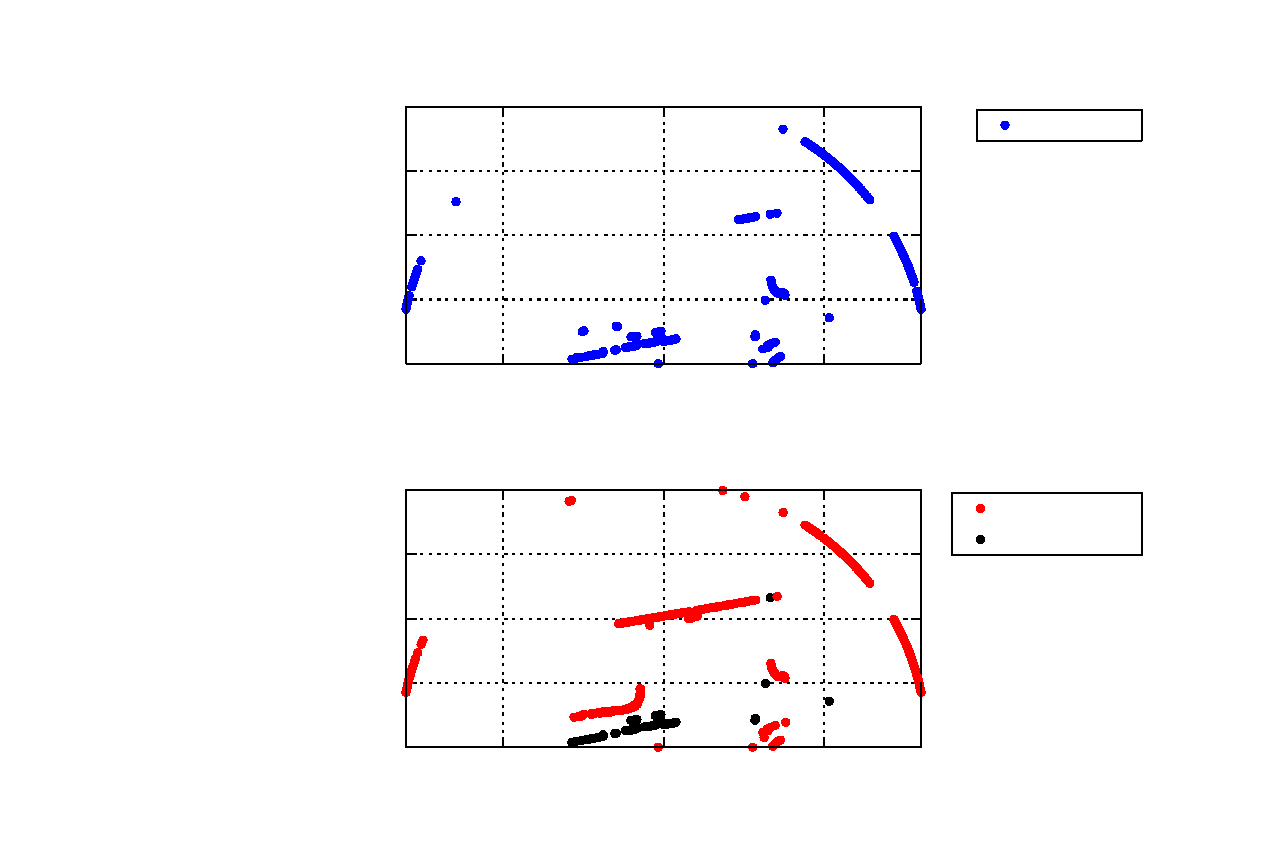
\includegraphics{fig/4/bg_process-inc}
\end{picture}%
\begin{picture}(600,400)(0,0)
\fontsize{10}{0}
\selectfont\put(233.334,228.516){\makebox(0,0)[t]{\textcolor[rgb]{0,0,0}{{-5000}}}}
\fontsize{10}{0}
\selectfont\put(310.5,228.516){\makebox(0,0)[t]{\textcolor[rgb]{0,0,0}{{0}}}}
\fontsize{10}{0}
\selectfont\put(387.666,228.516){\makebox(0,0)[t]{\textcolor[rgb]{0,0,0}{{5000}}}}
\fontsize{10}{0}
\selectfont\put(182.036,233.535){\makebox(0,0)[r]{\textcolor[rgb]{0,0,0}{{0}}}}
\fontsize{10}{0}
\selectfont\put(182.036,264.401){\makebox(0,0)[r]{\textcolor[rgb]{0,0,0}{{2000}}}}
\fontsize{10}{0}
\selectfont\put(182.036,295.267){\makebox(0,0)[r]{\textcolor[rgb]{0,0,0}{{4000}}}}
\fontsize{10}{0}
\selectfont\put(182.036,326.134){\makebox(0,0)[r]{\textcolor[rgb]{0,0,0}{{6000}}}}
\fontsize{10}{0}
\selectfont\put(182.036,357){\makebox(0,0)[r]{\textcolor[rgb]{0,0,0}{{8000}}}}
\fontsize{10}{0}
\selectfont\put(310.5,367){\makebox(0,0)[b]{\textcolor[rgb]{0,0,0}{{Raw laser data}}}}
\fontsize{10}{0}
\selectfont\put(488,348.095){\makebox(0,0)[l]{\textcolor[rgb]{0,0,0}{{Raw data}}}}
\fontsize{10}{0}
\selectfont\put(233.334,44.516){\makebox(0,0)[t]{\textcolor[rgb]{0,0,0}{{-5000}}}}
\fontsize{10}{0}
\selectfont\put(310.5,44.516){\makebox(0,0)[t]{\textcolor[rgb]{0,0,0}{{0}}}}
\fontsize{10}{0}
\selectfont\put(387.666,44.516){\makebox(0,0)[t]{\textcolor[rgb]{0,0,0}{{5000}}}}
\fontsize{10}{0}
\selectfont\put(182.036,49.5349){\makebox(0,0)[r]{\textcolor[rgb]{0,0,0}{{0}}}}
\fontsize{10}{0}
\selectfont\put(182.036,80.4012){\makebox(0,0)[r]{\textcolor[rgb]{0,0,0}{{2000}}}}
\fontsize{10}{0}
\selectfont\put(182.036,111.267){\makebox(0,0)[r]{\textcolor[rgb]{0,0,0}{{4000}}}}
\fontsize{10}{0}
\selectfont\put(182.036,142.134){\makebox(0,0)[r]{\textcolor[rgb]{0,0,0}{{6000}}}}
\fontsize{10}{0}
\selectfont\put(182.036,173){\makebox(0,0)[r]{\textcolor[rgb]{0,0,0}{{8000}}}}
\fontsize{10}{0}
\selectfont\put(310.5,183){\makebox(0,0)[b]{\textcolor[rgb]{0,0,0}{{Background model and extracted foreground}}}}
\fontsize{10}{0}
\selectfont\put(476.214,164.095){\makebox(0,0)[l]{\textcolor[rgb]{0,0,0}{{Background}}}}
\fontsize{10}{0}
\selectfont\put(476.214,149.175){\makebox(0,0)[l]{\textcolor[rgb]{0,0,0}{{Foreground}}}}
\end{picture}
